%
% T�TULO DEL CAP�TULO
%
\chapter[RANSAC]{
	Random Sample Consensus
	\label{chapter_8}
}

RANSAC is an abbreviation for ``RANdom SAmple Consensus''. This is an iterative method to estimate parameters of a mathematical model from a set of observed points which can contain outliers. This is a non-deterministic algorithm, since we are not able to guarantee that it will produce a correct result. The probability of reaching a reasonable result will improve as the number of iterations increases. The algorithm was first published in \cite{ransac}.

The basic assumption is that the data contains \textit{inliers}\footnote{Data whose distribution can be estimated by some model.}, though it may contain noise and \textit{outliers}\footnote{Data that does not fit the model.}. Outliers can come from errors or imprecise measurements, extreme values of noise, etc. RANSAC assumes that given a set of inliers, there should exist a procedure that can estimate the unknown parameters of a model that will fit this data (see \autoref{RANSAC}).

\begin{figure}[h]
	\centering
	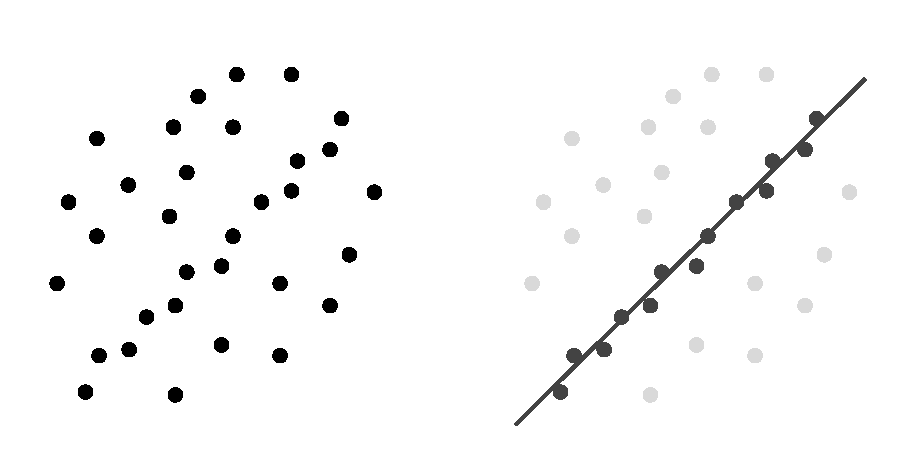
\includegraphics[scale=0.8]{figures/RANSAC.pdf}
	\caption[RANSAC example]{
		A set of points with many inliers in which a line is to be fitted (\textbf{left}).  Resulting fitted line using RANSAC, in which outliers have no influence in the result (\textbf{right}).
	}
	\label{RANSAC}
\end{figure}

\section[Original algorithm]{Original algorithm}

Unlike other estimation techniques, RANSAC generates candidate solutions using the minimum number of points required to fit the model parameters. RANSAC instead of using as much of the data as possible and then eliminate the outliers, uses the smallest set possible and then tries to enlarge this subset with coherent points. The basic algorithm can be summed up in the following steps: 

\begin{enumerate}
	\item Select randomly the minimum subset of points to determine the model parameters.
	\item Solve for the parameters of the model (i.e. with a least squares method).
	\item Test how many points from the complete dataset fit with a predefined tolerance $\epsilon$.
	\item If the fraction of inliers over the total number of points is sufficiently good, then the model is re-estimated (since it was only estimated using the initial inliers).
	\item Finally, the model is evaluated by estimating the error of the inliers relative to the model.
\end{enumerate}

This procedure is repeated a certain number of times, each time producing either a new model which is either rejected because too few points are classified as inliers or a better model together with its error measure. In the latter case, we keep the refined model if its error is lower than the last saved model.

The algorithm will stop when it reaches $N$ iterations or when the model reaches a desired error measure. $N$ can be calculated to ensure that the probability $p$ (usually 0.99) of one of the subsets of random samples will not contain an outlier. Being $u$ the probability that any selected point is an inlier and $v = 1 - u$ the probability of observing an outlier. $N$ iterations of the minimum number of points $m$ are required:

\begin{equation}\label{eq:depth} 1 - p = (1 - u^m)^N \end{equation}

After solving for $N$ we will obtain the necessary number of iterations:

\begin{equation}\label{eq:depth} N = \frac{log(1 - p)}{log(1 - (1 - v) ^ m)} \end{equation}

Since our objective is estimating primitives in real-time, we will let the user choose this parameter so that computational time is not too high.

An advantage of RANSAC is the robust estimation of the model parameters (it can estimate the parameters even when a significant number of outliers is present). But, a disadvantage of RANSAC is that there is no upper bound on the time that it would take to compute the correct model parameters. Another disadvantage is that it can only estimate one model at a time, if two or more instances of the model exist, RANSAC will fail to find either of them.

 


